
\subsection{Tasks Correctness}
\label{cp6:correctness}



When assisted by a tool able to automatically highlight text identified as relevant to a task, we expect that a developer can produce a solution 
that is equally or more correct than the solution of a developer who attempted a task without tool support. 


To compute how correct a participant's solution is, 
we compile their code and run it against a set of 10 test cases that check whether it produces the correct output for each given test input. 
Hence, \textit{correctness} represents the number of passing test cases of a solution (Equation~\ref{eq:cp6-correctness}).
For example, if the solution of a participant passes 7 out of 10 test cases, we would assign a 
correctness score of $7$ to this solution. 
A solution with compile errors has a correctness score of $0$.


\smallskip
\begin{small}


\begin{equation}
    Correctness = \text{\textit{\# of passing test cases}}
    \label{eq:cp6-correctness}
\end{equation}
\end{small}



\smallskip


From all submitted solutions (24 manual and 24 tool-assisted ones), two 
solutions from tool-assisted tasks had compile errors or failed all test cases. 
One of the solutions that failed all test cases
was from a participant who indicated that they decided to not finish their tool-assisted task due to time constraints; the other, from an Exception thrown in a solution that misused the \texttt{geopy} module. We do not ignore these two solutions when reporting results.


Figure~\ref{fig:correctness-overall} and 
show results for the correctness scores of solutions submitted by participants
who performed a task with and without tool support. 
On average both manual and tool-assisted solutions have a correctness score of $7$.
The notable difference between manual and tool-assisted solutions appear in the 1st quartile of the data which suggests that, 
when assisted by our tool, participants had slightly more correct solutions. 
However, comparison of the correctness scores of manual and tool-assisted solutions via a 
Wilcoxon signed-rank test suggests we cannot draw statistically significant conclusions
based on our data.



% (Table~\ref{tbl:correctness-overall})



% \begin{table}
\caption{Descriptive statistics for correctness}
\label{tbl:correctness-overall}
\centering    
% \begin{scriptsize}
\begin{threeparttable}
\begin{tabular}{lcccccc}

& \textbf{min} & \textbf{1st Qu.} 
& \textbf{median} & \textbf{mean}
& \textbf{3rd Qu.} & \textbf{max}
\\ 
\hline

Manual & 2.0 &    4.0   &  7.5   &  7.0   &  9.0   & 10.0
\\

Tool-assisted  &  0.0  & 5.5 &  8.0 &  7.0 &  9.0 & 10.0
\\


\hline

\end{tabular}
\end{threeparttable}
% \end{scriptsize}
\end{table}







\label{fig:correctness-overall}


\begin{figure}[h!]
    \centering
    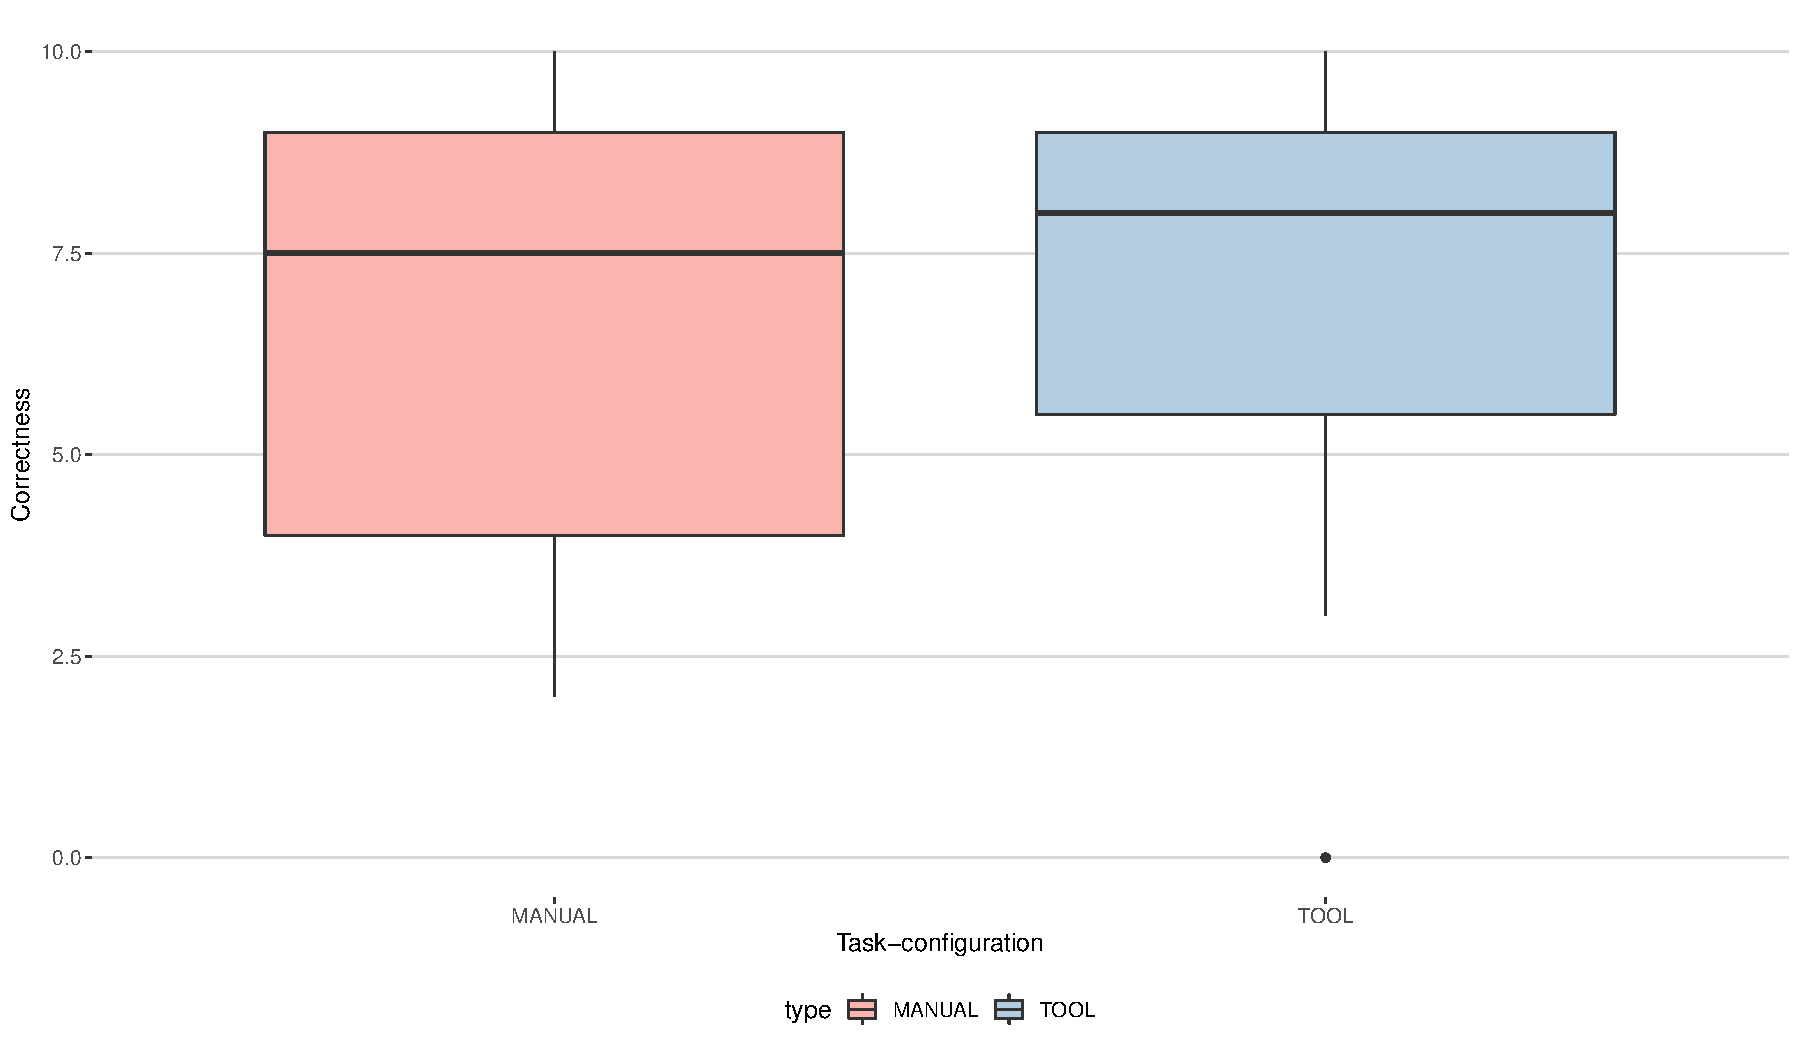
\includegraphics[width=\textwidth]{cp6/correctness_aggregated.pdf}
    \caption{Comparison of correctness of solutions for manual and tool-assisted tasks}
    \label{fig:correctness-overall}
\end{figure}



% Figure~\ref{fig:correctness-by-task} details results per task.



\begin{figure}[h!]
    \centering
    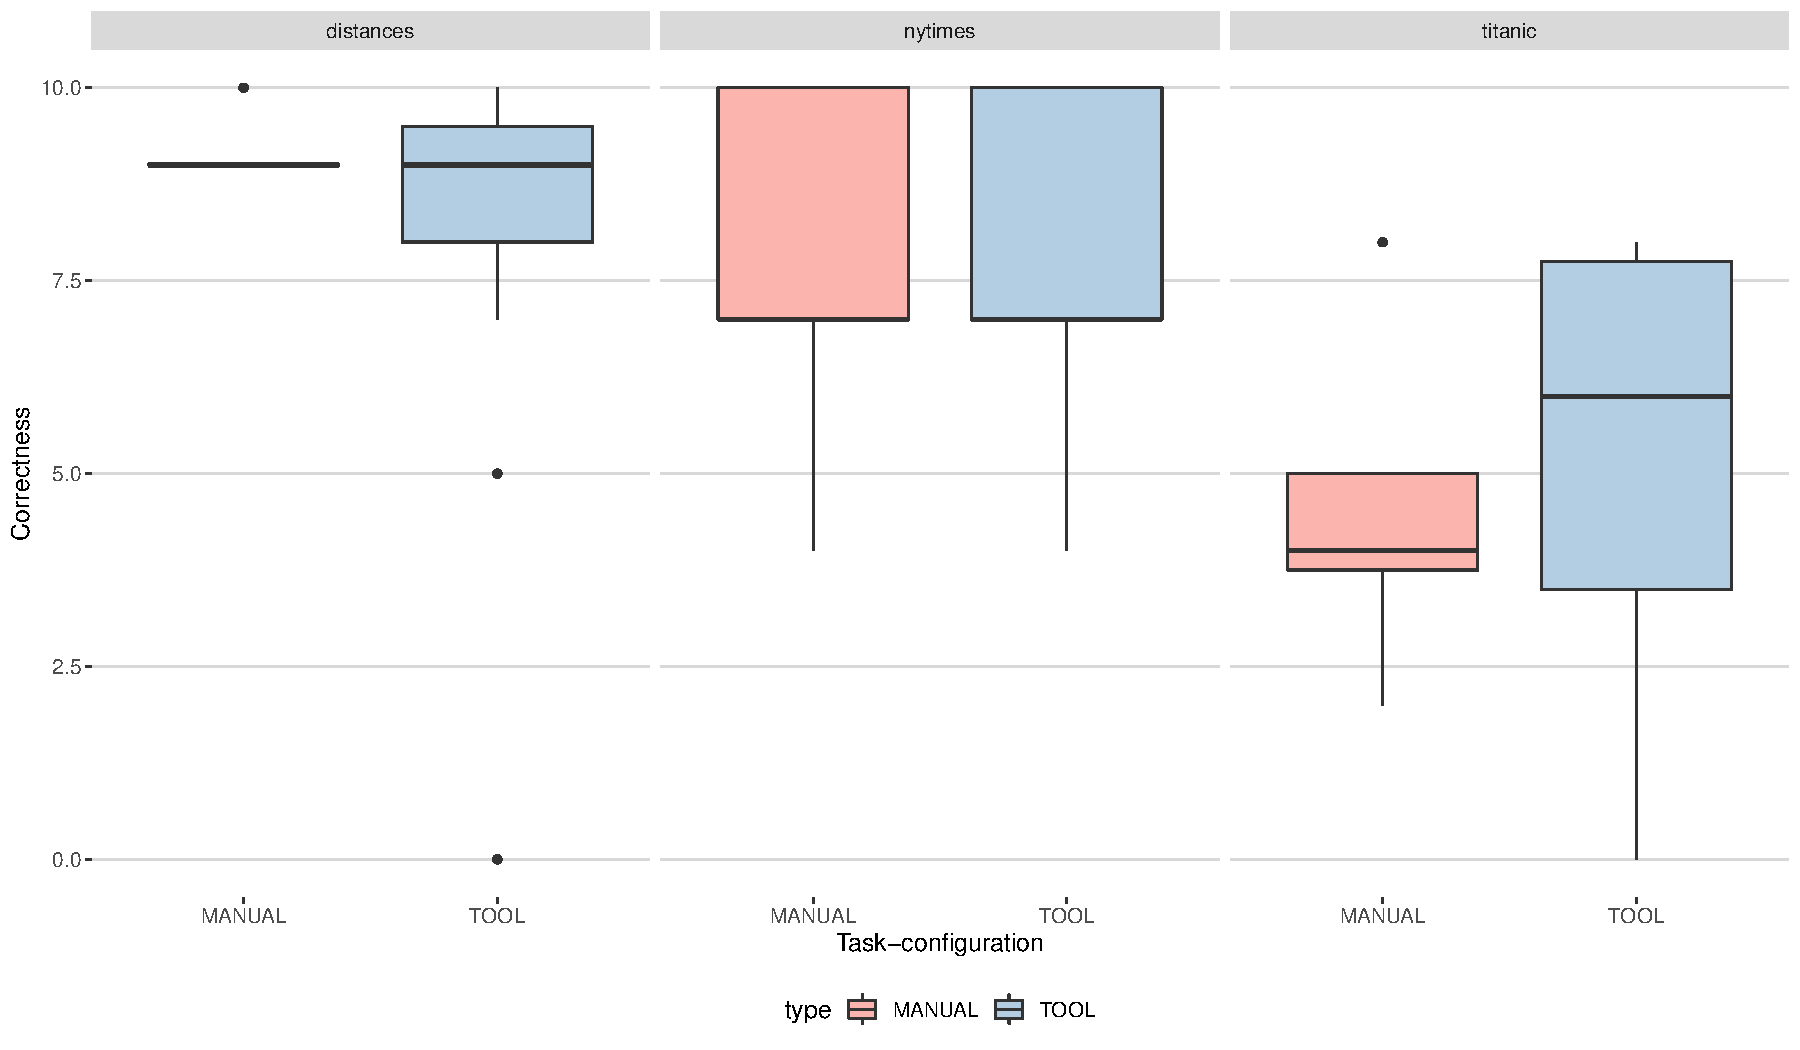
\includegraphics[width=\textwidth]{cp6/correctness_overall.pdf}
    \caption{Detailed comparison of correctness of solutions for manual and tool-assisted tasks}
    \label{fig:correctness-by-task}
\end{figure}

